%% bare_conf.tex
%% V1.3
%% 2007/01/11
%% by Michael Shell
%% See:
%% http://www.michaelshell.org/
%% for current contact information.
%%
%% This is a skeleton file demonstrating the use of IEEEtran.cls
%% (requires IEEEtran.cls version 1.7 or later) with an IEEE conference paper.
%%
%% Support sites:
%% http://www.michaelshell.org/tex/ieeetran/
%% http://www.ctan.org/tex-archive/macros/latex/contrib/IEEEtran/
%% and
%% http://www.ieee.org/

%%*************************************************************************
%% Legal Notice:
%% This code is offered as-is without any warranty either expressed or
%% implied; without even the implied warranty of MERCHANTABILITY or
%% FITNESS FOR A PARTICULAR PURPOSE! 
%% User assumes all risk.
%% In no event shall IEEE or any contributor to this code be liable for
%% any damages or losses, including, but not limited to, incidental,
%% consequential, or any other damages, resulting from the use or misuse
%% of any information contained here.
%%
%% All comments are the opinions of their respective authors and are not
%% necessarily endorsed by the IEEE.
%%
%% This work is distributed under the LaTeX Project Public License (LPPL)
%% ( http://www.latex-project.org/ ) version 1.3, and may be freely used,
%% distributed and modified. A copy of the LPPL, version 1.3, is included
%% in the base LaTeX documentation of all distributions of LaTeX released
%% 2003/12/01 or later.
%% Retain all contribution notices and credits.
%% ** Modified files should be clearly indicated as such, including  **
%% ** renaming them and changing author support contact information. **
%%
%% File list of work: IEEEtran.cls, IEEEtran_HOWTO.pdf, bare_adv.tex,
%%                    bare_conf.tex, bare_jrnl.tex, bare_jrnl_compsoc.tex
%%*************************************************************************

% *** Authors should verify (and, if needed, correct) their LaTeX system  ***
% *** with the testflow diagnostic prior to trusting their LaTeX platform ***
% *** with production work. IEEE's font choices can trigger bugs that do  ***
% *** not appear when using other class files.                            ***
% The testflow support page is at:
% http://www.michaelshell.org/tex/testflow/



% Note that the a4paper option is mainly intended so that authors in
% countries using A4 can easily print to A4 and see how their papers will
% look in print - the typesetting of the document will not typically be
% affected with changes in paper size (but the bottom and side margins will).
% Use the testflow package mentioned above to verify correct handling of
% both paper sizes by the user's LaTeX system.
%
% Also note that the "draftcls" or "draftclsnofoot", not "draft", option
% should be used if it is desired that the figures are to be displayed in
% draft mode.
%
\documentclass[conference]{IEEEtran}
\usepackage{graphicx}
% Add the compsoc option for Computer Society conferences.
%
% If IEEEtran.cls has not been installed into the LaTeX system files,
% manually specify the path to it like:
% \documentclass[conference]{../sty/IEEEtran}





% Some very useful LaTeX packages include:
% (uncomment the ones you want to load)


% *** MISC UTILITY PACKAGES ***
%
%\usepackage{ifpdf}
% Heiko Oberdiek's ifpdf.sty is very useful if you need conditional
% compilation based on whether the output is pdf or dvi.
% usage:
% \ifpdf
%   % pdf code
% \else
%   % dvi code
% \fi
% The latest version of ifpdf.sty can be obtained from:
% http://www.ctan.org/tex-archive/macros/latex/contrib/oberdiek/
% Also, note that IEEEtran.cls V1.7 and later provides a builtin
% \ifCLASSINFOpdf conditional that works the same way.
% When switching from latex to pdflatex and vice-versa, the compiler may
% have to be run twice to clear warning/error messages.






% *** CITATION PACKAGES ***
%
%\usepackage{cite}
% cite.sty was written by Donald Arseneau
% V1.6 and later of IEEEtran pre-defines the format of the cite.sty package
% \cite{} output to follow that of IEEE. Loading the cite package will
% result in citation numbers being automatically sorted and properly
% "compressed/ranged". e.g., [1], [9], [2], [7], [5], [6] without using
% cite.sty will become [1], [2], [5]--[7], [9] using cite.sty. cite.sty's
% \cite will automatically add leading space, if needed. Use cite.sty's
% noadjust option (cite.sty V3.8 and later) if you want to turn this off.
% cite.sty is already installed on most LaTeX systems. Be sure and use
% version 4.0 (2003-05-27) and later if using hyperref.sty. cite.sty does
% not currently provide for hyperlinked citations.
% The latest version can be obtained at:
% http://www.ctan.org/tex-archive/macros/latex/contrib/cite/
% The documentation is contained in the cite.sty file itself.






% *** GRAPHICS RELATED PACKAGES ***
%
\ifCLASSINFOpdf
  % \usepackage[pdftex]{graphicx}
  % declare the path(s) where your graphic files are
  % \graphicspath{{../pdf/}{../jpeg/}}
  % and their extensions so you won't have to specify these with
  % every instance of \includegraphics
  % \DeclareGraphicsExtensions{.pdf,.jpeg,.png}
\else
  % or other class option (dvipsone, dvipdf, if not using dvips). graphicx
  % will default to the driver specified in the system graphics.cfg if no
  % driver is specified.
  % \usepackage[dvips]{graphicx}
  % declare the path(s) where your graphic files are
  % \graphicspath{{../eps/}}
  % and their extensions so you won't have to specify these with
  % every instance of \includegraphics
  % \DeclareGraphicsExtensions{.eps}
\fi
% graphicx was written by David Carlisle and Sebastian Rahtz. It is
% required if you want graphics, photos, etc. graphicx.sty is already
% installed on most LaTeX systems. The latest version and documentation can
% be obtained at: 
% http://www.ctan.org/tex-archive/macros/latex/required/graphics/
% Another good source of documentation is "Using Imported Graphics in
% LaTeX2e" by Keith Reckdahl which can be found as epslatex.ps or
% epslatex.pdf at: http://www.ctan.org/tex-archive/info/
%
% latex, and pdflatex in dvi mode, support graphics in encapsulated
% postscript (.eps) format. pdflatex in pdf mode supports graphics
% in .pdf, .jpeg, .png and .mps (metapost) formats. Users should ensure
% that all non-photo figures use a vector format (.eps, .pdf, .mps) and
% not a bitmapped formats (.jpeg, .png). IEEE frowns on bitmapped formats
% which can result in "jaggedy"/blurry rendering of lines and letters as
% well as large increases in file sizes.
%
% You can find documentation about the pdfTeX application at:
% http://www.tug.org/applications/pdftex





% *** MATH PACKAGES ***
%
%\usepackage[cmex10]{amsmath}
% A popular package from the American Mathematical Society that provides
% many useful and powerful commands for dealing with mathematics. If using
% it, be sure to load this package with the cmex10 option to ensure that
% only type 1 fonts will utilized at all point sizes. Without this option,
% it is possible that some math symbols, particularly those within
% footnotes, will be rendered in bitmap form which will result in a
% document that can not be IEEE Xplore compliant!
%
% Also, note that the amsmath package sets \interdisplaylinepenalty to 10000
% thus preventing page breaks from occurring within multiline equations. Use:
%\interdisplaylinepenalty=2500
% after loading amsmath to restore such page breaks as IEEEtran.cls normally
% does. amsmath.sty is already installed on most LaTeX systems. The latest
% version and documentation can be obtained at:
% http://www.ctan.org/tex-archive/macros/latex/required/amslatex/math/





% *** SPECIALIZED LIST PACKAGES ***
%
%\usepackage{algorithmic}
% algorithmic.sty was written by Peter Williams and Rogerio Brito.
% This package provides an algorithmic environment fo describing algorithms.
% You can use the algorithmic environment in-text or within a figure
% environment to provide for a floating algorithm. Do NOT use the algorithm
% floating environment provided by algorithm.sty (by the same authors) or
% algorithm2e.sty (by Christophe Fiorio) as IEEE does not use dedicated
% algorithm float types and packages that provide these will not provide
% correct IEEE style captions. The latest version and documentation of
% algorithmic.sty can be obtained at:
% http://www.ctan.org/tex-archive/macros/latex/contrib/algorithms/
% There is also a support site at:
% http://algorithms.berlios.de/index.html
% Also of interest may be the (relatively newer and more customizable)
% algorithmicx.sty package by Szasz Janos:
% http://www.ctan.org/tex-archive/macros/latex/contrib/algorithmicx/




% *** ALIGNMENT PACKAGES ***
%
%\usepackage{array}
% Frank Mittelbach's and David Carlisle's array.sty patches and improves
% the standard LaTeX2e array and tabular environments to provide better
% appearance and additional user controls. As the default LaTeX2e table
% generation code is lacking to the point of almost being broken with
% respect to the quality of the end results, all users are strongly
% advised to use an enhanced (at the very least that provided by array.sty)
% set of table tools. array.sty is already installed on most systems. The
% latest version and documentation can be obtained at:
% http://www.ctan.org/tex-archive/macros/latex/required/tools/


%\usepackage{mdwmath}
%\usepackage{mdwtab}
% Also highly recommended is Mark Wooding's extremely powerful MDW tools,
% especially mdwmath.sty and mdwtab.sty which are used to format equations
% and tables, respectively. The MDWtools set is already installed on most
% LaTeX systems. The lastest version and documentation is available at:
% http://www.ctan.org/tex-archive/macros/latex/contrib/mdwtools/


% IEEEtran contains the IEEEeqnarray family of commands that can be used to
% generate multiline equations as well as matrices, tables, etc., of high
% quality.


%\usepackage{eqparbox}
% Also of notable interest is Scott Pakin's eqparbox package for creating
% (automatically sized) equal width boxes - aka "natural width parboxes".
% Available at:
% http://www.ctan.org/tex-archive/macros/latex/contrib/eqparbox/





% *** SUBFIGURE PACKAGES ***
%\usepackage[tight,footnotesize]{subfigure}
% subfigure.sty was written by Steven Douglas Cochran. This package makes it
% easy to put subfigures in your figures. e.g., "Figure 1a and 1b". For IEEE
% work, it is a good idea to load it with the tight package option to reduce
% the amount of white space around the subfigures. subfigure.sty is already
% installed on most LaTeX systems. The latest version and documentation can
% be obtained at:
% http://www.ctan.org/tex-archive/obsolete/macros/latex/contrib/subfigure/
% subfigure.sty has been superceeded by subfig.sty.



%\usepackage[caption=false]{caption}
%\usepackage[font=footnotesize]{subfig}
% subfig.sty, also written by Steven Douglas Cochran, is the modern
% replacement for subfigure.sty. However, subfig.sty requires and
% automatically loads Axel Sommerfeldt's caption.sty which will override
% IEEEtran.cls handling of captions and this will result in nonIEEE style
% figure/table captions. To prevent this problem, be sure and preload
% caption.sty with its "caption=false" package option. This is will preserve
% IEEEtran.cls handing of captions. Version 1.3 (2005/06/28) and later 
% (recommended due to many improvements over 1.2) of subfig.sty supports
% the caption=false option directly:
%\usepackage[caption=false,font=footnotesize]{subfig}
%
% The latest version and documentation can be obtained at:
% http://www.ctan.org/tex-archive/macros/latex/contrib/subfig/
% The latest version and documentation of caption.sty can be obtained at:
% http://www.ctan.org/tex-archive/macros/latex/contrib/caption/




% *** FLOAT PACKAGES ***
%
%\usepackage{fixltx2e}
% fixltx2e, the successor to the earlier fix2col.sty, was written by
% Frank Mittelbach and David Carlisle. This package corrects a few problems
% in the LaTeX2e kernel, the most notable of which is that in current
% LaTeX2e releases, the ordering of single and double column floats is not
% guaranteed to be preserved. Thus, an unpatched LaTeX2e can allow a
% single column figure to be placed prior to an earlier double column
% figure. The latest version and documentation can be found at:
% http://www.ctan.org/tex-archive/macros/latex/base/



%\usepackage{stfloats}
% stfloats.sty was written by Sigitas Tolusis. This package gives LaTeX2e
% the ability to do double column floats at the bottom of the page as well
% as the top. (e.g., "\begin{figure*}[!b]" is not normally possible in
% LaTeX2e). It also provides a command:
%\fnbelowfloat
% to enable the placement of footnotes below bottom floats (the standard
% LaTeX2e kernel puts them above bottom floats). This is an invasive package
% which rewrites many portions of the LaTeX2e float routines. It may not work
% with other packages that modify the LaTeX2e float routines. The latest
% version and documentation can be obtained at:
% http://www.ctan.org/tex-archive/macros/latex/contrib/sttools/
% Documentation is contained in the stfloats.sty comments as well as in the
% presfull.pdf file. Do not use the stfloats baselinefloat ability as IEEE
% does not allow \baselineskip to stretch. Authors submitting work to the
% IEEE should note that IEEE rarely uses double column equations and
% that authors should try to avoid such use. Do not be tempted to use the
% cuted.sty or midfloat.sty packages (also by Sigitas Tolusis) as IEEE does
% not format its papers in such ways.





% *** PDF, URL AND HYPERLINK PACKAGES ***
%
%\usepackage{url}
% url.sty was written by Donald Arseneau. It provides better support for
% handling and breaking URLs. url.sty is already installed on most LaTeX
% systems. The latest version can be obtained at:
% http://www.ctan.org/tex-archive/macros/latex/contrib/misc/
% Read the url.sty source comments for usage information. Basically,
% \url{my_url_here}.





% *** Do not adjust lengths that control margins, column widths, etc. ***
% *** Do not use packages that alter fonts (such as pslatex).         ***
% There should be no need to do such things with IEEEtran.cls V1.6 and later.
% (Unless specifically asked to do so by the journal or conference you plan
% to submit to, of course. )


% correct bad hyphenation here
\hyphenation{op-tical net-works semi-conduc-tor}


\begin{document}
%
% paper title
% can use linebreaks \\ within to get better formatting as desired
\title{A Machine Learning Approach to Detect Phishing Websites}


% author names and affiliations
% use a multiple column layout for up to three different
% affiliations
\author{\IEEEauthorblockN{Arnab Sen Sharma Api}
\IEEEauthorblockA{Lecturer\\
Department of Computer\\Science \& Engineering, SUST\\
Email: arnab-cse@sust.edu}
\and
\IEEEauthorblockN{Md. Sabbir Sattar Mukit}
\IEEEauthorblockA{Department of Computer\\Science \& Engineering, SUST\\
Email: sabbir.mukit379@gmail.com}
\and
\IEEEauthorblockN{Nirjas Mohammad Jakilim}
\IEEEauthorblockA{Department of Computer\\Science \& Engineering, SUST\\
Email: nirzashzakilim@gmail.com}}

% conference papers do not typically use \thanks and this command
% is locked out in conference mode. If really needed, such as for
% the acknowledgment of grants, issue a \IEEEoverridecommandlockouts
% after \documentclass

% for over three affiliations, or if they all won't fit within the width
% of the page, use this alternative format:
% 
%\author{\IEEEauthorblockN{Michael Shell\IEEEauthorrefmark{1},
%Homer Simpson\IEEEauthorrefmark{2},
%James Kirk\IEEEauthorrefmark{3}, 
%Montgomery Scott\IEEEauthorrefmark{3} and
%Eldon Tyrell\IEEEauthorrefmark{4}}
%\IEEEauthorblockA{\IEEEauthorrefmark{1}School of Electrical and Computer Engineering\\
%Georgia Institute of Technology,
%Atlanta, Georgia 30332--0250\\ Email: see http://www.michaelshell.org/contact.html}
%\IEEEauthorblockA{\IEEEauthorrefmark{2}Twentieth Century Fox, Springfield, USA\\
%Email: homer@thesimpsons.com}
%\IEEEauthorblockA{\IEEEauthorrefmark{3}Starfleet Academy, San Francisco, California 96678-2391\\
%Telephone: (800) 555--1212, Fax: (888) 555--1212}
%\IEEEauthorblockA{\IEEEauthorrefmark{4}Tyrell Inc., 123 Replicant Street, Los Angeles, California 90210--4321}}




% use for special paper notices
%\IEEEspecialpapernotice{(Invited Paper)}




% make the title area
\maketitle


\begin{abstract}
%\boldmath
The goal of our project is to implement a system to detect phishing websites using machine learning. The result of our project will be a
software product which uses machine learning algorithm to detect
phishing URLs. Phishing is the technique of stealing user
credentials and sensitive data from users by masquerading as
the original website. In phishing, the user is provided with a
mirror website which is identical to the legitimate one but with
malicious code or technique to extract and send user credentials to phishers.
Phishing attacks can lead to huge financial losses for customers
of banking or many financial business services. The traditional approach to
detect phishing has been either to use a blacklist of known phishing links or heuristically evaluate the attributes in a suspected phishing page to detect the presence of malicious codes. The drawback to heuristic approach is poor accuracy and low adaptability to new phishing links. We plan to use machine learning to overcome these drawbacks by implementing some classification algorithms and comparing the performance of these algorithms on our dataset.We will test algorithms such as SVM, Random Forests and Neural Networks on a dataset of phishing links from UCI Machine Learning repository and pick the best model to develop a chrome browser extension.
\end{abstract}
% IEEEtran.cls defaults to using nonbold math in the Abstract.
% This preserves the distinction between vectors and scalars. However,
% if the conference you are submitting to favors bold math in the abstract,
% then you can use LaTeX's standard command \boldmath at the very start
% of the abstract to achieve this. Many IEEE journals/conferences frown on
% math in the abstract anyway.

% no keywords




% For peer review papers, you can put extra information on the cover
% page as needed:
% \ifCLASSOPTIONpeerreview
% \begin{center} \bfseries EDICS Category: 3-BBND \end{center}
% \fi
%
% For peerreview papers, this IEEEtran command inserts a page break and
% creates the second title. It will be ignored for other modes.
\IEEEpeerreviewmaketitle



\section{Introduction}
% no \IEEEPARstart
\par Financial services like banking services are now going online to make people's life easy and simple. Thus the security of this online services is
very important. One of the biggest threats to web security
is Phishing. Phishing is the technique of extracting user
credentials by masquerading as a genuine website or service
over the web. There are various types of phishing attacks
such as Spear phishing, which targets specific individuals
or companies, Clone phishing is a type of phishing where
an original mail with an attachment or link is copied into
a new mail with a different (possibly malicious) attachment
or link etc. Phishing can lead to huge financial
losses. For example, the Microsoft Consumer Safer Index
(MCSI) report for 2014 has estimated the annual worldwide
impact of Phishing and other identity thefts to be nearly USD
5 Billion [1]. Similarly, the IRS has warned of a surge in
phishing attacks with over 400\% increase in reported cases [2].
\par Several solutions have been proposed to prevent phishing
ranging from educating the web users to tackle phishing attacks. The conventional approach to phishing detection has not been successful because of the diverse and
evolving nature of phishing attacks. For instance, in January
2007, the total number of unique phishing reports submitted
to the Anti-Phishing Working Group (APWG) was 29,930.
Compared to the previous peak in June 2006, the number
of submitted reports increased by 5\% [3]. This happened
despite taking preventive measure to detect phishing. Upon
investigation, it was found that each phishing attack was
different from the other one. Thus it becomes imperative to
find a way to adapt our phishing detection techniques.
\par Machine learning algorithms, which make a system learn
new patterns from data, are an ideal solution to the problem of
phishing detection. Although there have been many papers in
recent years which have attempted to detect phishing attacks
using machine learning, we intend to go one first step further
and build a software tool which can be easily deployed in
end user systems to detect phishing attacks.
\par For our project, we will experiment with three machine
learning algorithms on a dataset of features that represent
attributes commonly associated with phishing pages. We'll then choose
the best model based on their performance and build a web
browser extension which will eventually be deployed to end
users.

\section{Related Work}
\par There are generally two approaches to detect phishing websites. One is the blacklist approach and the other is heuristic approach. The blacklist approach is involving a publicly available database of already reported blacklisted site. Then to detect new phishing sites the system just matches the new site with the previous blacklisted site. The main drawback with this approach is that a new
phishing site has to be detected first before it can be reported.
As phishers become more sophisticated with their phishing
attacks, it becomes more difficult to detect those attacks.Also one has to maintain huge database costs to implement such system. The second approach is heuristic approach. This method works by analyzing the source
code of a suspected phishing web page and identify attributes
commonly associated with phishing sites. This approach is
better than the blacklist method as we can potentially detect
new phishing attacks within minutes of their launch. but because of the diverse nature of phishing attacks it has become increasingly difficult to detect new attack
patterns.Traditionally, the heuristic evaluation of the web page
source code involved maintaining a count of identified phishing
attributes and setting threshold for that count using trial and
error, above which the page was considered a phishing site.
As it is obvious, the hardcoding of such thresholds inherently
make it difficult for the phishing detection system to adapt
to new attack patterns. That's why we use machine learning to train
the system to detect phishing attacks and relearn from the data
whenever a new phishing attack pattern is uncovered. There
are sufficient literatures in recent years employing machine
learning algorithms to the problem of phishing detection. In
[3], for example, the work done by Chandrasekaran et al.
describes a technique to classify phishing emails based on their
structural properties such as style markers and the structure
of the subject line, etc. They used Simulated Annealing for
feature selection and Information Gain to rank the features
based on their relevance on a dataset of 100 phishing emails
and 100 legitimate emails. Later they used Support Vector
Machines to classify the emails as phishing and legitimate
based on their chosen features, getting an accuracy of 95\%.
The paper [3] also describes the approach taken by Fette et
al., where they compared commonly used learning algorithms
on a dataset of detected phishing emails composed of 860
phishing emails and 6950 legitimate emails. They hand picked
ten features and used Random Forests algorithm on the dataset
which provided an accuracy of 97\% with a false positive rate
of 0.1\%.
\section{Proposed Approach}
We propose to use machine learning to overcome the
drawbacks associated with the traditional approaches. The basic idea of our project is to use machine learning algorithms on available dataset of phishing
pages to generate a model which can be used to make
classifications in real time if a given web page is a phishing
page or a legitimate webpage. We intend to integrate the
learned model into a software tool which can be deployed
easily to end users. For this reason we have chosen to implement a machine learning
algorithm from scratch using JavaScript and build a Chrome Extension. We choose Chrome Extension because it's most popular among the users. Also the Chrome Web Store enable us to deploy our extension to chrome users.
\par In order to successfully implement this project, we need to
consider three constraints when choosing the machine learning
algorithm for our product. First, the accuracy of the trained
model should be high, as a product being used by end users
in the real world should not give wrong results. Second,
the algorithm which is being implemented should be able to
make classifications in real-time; i.e. have very low execution
time and also use less computational resources. Third, false
positives and false negatives are important considerations when
choosing a machine learning algorithm for the problem of
phishing detection. This is because a user should not be
wrongly led to believe that a phishing website is legitimate.
Thus, we should look at these three constraints when selecting
our phishing detection classifier.
\section{Dataset}
To evaluate the machine learning algorithms we take our Dataset from UCI machine learning repository. It consists of 11,055 URLs (instances)
with 6157 phishing instances and 4898 legitimate instances.
Each instance contains 16 features. Each feature is associated
with a rule. If the rule satisfies, it is termed as phishing. If
the rule doesn’t satisfy then it is termed as legitimate. The
features take three discrete values. ‘1’ if the rule is satisfied,
‘0’ if the rule is partially satisfied, ‘-1’ if the rule is not
satisfied.
\par Our features represented by the training dataset can be
classified into four categories;
i) Address Bar based features
ii) Abnormal based features
iii) HTML and JavaScript based features
iv) Domain based features
\subsection{Address bar based features}
\par 1.1 Contains IP address: If the domain of the URL of
the suspected web page contains IP address, then we take
it as a phishing page. eg: http:160.100.45.151facebook.html or
http:x100.0xFA.0xCE.0xBOOK.caindex.html

\par 1.2 Using Long URL to hide suspicious part: Phishers often use long urls to hide suspicious part and make users confused by including legitimate site's url.
eg: facebookverify.000webhost.com/accountsverify.facebook.com.html

\par 1.3 Use of URL shortening services: A shortened url always hides the real suspicious url. So, hackers often use it to distract users. Therefore, we
set the rule that if the URL has been shortened using a URL
shortening service then it is a phishing page and legitimate
otherwise.

\par 1.4 Use of "@" symbol: Needs verification The "@"
symbol is a reserved keyword according to Web standards.
So the presence of "@" in a URL is suspicious and the web
page is taken as phishing and legitimate otherwise.

\par 1.5 Redirection with "//": The presence of "//" in the URL
path indicates the page will be redirected to another page. If
the position of "//" in the URL is greater than seven then it is
a phishing site and legitimate otherwise.

\par Adding prefix or suffix separated by "-" to the domain:
Phishers sometimes add a prefix or suffix to the domain with "-" to
give the resemblence of a geniune site. eg: service-verification-paypal-com.cct.com

\par 1.7 Sub domains and multi sub domains: If a URL has
more than three dots in the domain part then it is considered
as a phishing site and legitimate otherwise. eg: passwordreset.facebook.com.scgt.com
\subsubsection{Abnormal based features}

\par 2.1 Request URL: A legitimate site usually has external
page objects such as images, animations, files, etc. be accessed
by a request URL which shares the same domain as the web
page URL. We classify sites which fail this rule as phishing.

\par 2.2 URL portion of anchor tag: We check if the domain
in the URL portion of all anchor tags match the main URL
of the page and if the anchor tag has only URL fragments or
JavaScript functions.

\par 2.3 Links in <meta>, <script> and <link> tags: We check
if the domain of the links in the <meta>, <script> and <link>
tags matches the domain in the mail URL.

\par 2.4 Server Form Handler (SFH): When a form is submitted,
some valid action must be taken. So if the action handler of a
form is empty or "about:blank" or if the domain of the action
URL is different from the domain of the main URL, then it is
taken as a phishing site.

\par 2.5 Submitting Information to Email: If the webpage contains
a "mailto:" function then it is taken as a phishing site
and legitimate otherwise.

\subsection{HTML and Javascript based features}
\par 3.1 Status bar customization: Phishers can modify the
status bar using JavaScript to show a legitimate URL. By
analyzing the "onMouseOver" events in the web page we can
determine if such a modification has occurred.

\par 3.2 Disabling right click option: Phishers can disable the
right click option to prevent the user from checking the source
code of the page. This is checked analyzing the source code.

\par 3.3 Using pop-up window: Legitimate sites rarely ask for
user info on a pop-up window, whereas phishing sites generally
use pop-up windows to get user info.

\par 3.4 Iframe redirection: Phishers also use Iframe tags with
invisible borders to get user info and redirect to the original
site. We analyze the source code to check if Iframe tags are
used.
\section{Machine Learning Implementation}
We have tested and trained supervised machine learning
algorithms on the training dataset. The following algorithms
were chosen based on their performance on classification
problems. The dataset was split into training and test set in
the ratio 7:3. We have given the result of our experiment on the result section.
\subsection{Random Forests}
\par Random forests are classifiers that combine many tree
predictors, where each tree depends on the values of a random
vector sampled independently. Furthermore, all trees in the
forest have the same distribution. To construct a tree, we
assume that n is the number of training observations and p
is the number of variables (features) in a training set. To
determine the decision node at a tree we choose k « p as
the number of variables to be selected. We select a bootstrap
sample from the n observations in the training set and use
the rest of the observations to estimate the error of the tree
in the testing phase. Thus, we randomly choose k variables
as a decision at a certain node in the tree and calculate
the best split based on the k variables in the training set.
Trees are always grown and never pruned compared to other
tree algorithms. Random forests can handle large number
of variables in a data set. Also, during the forest building
process they generate an internal unbiased estimate of the
generalization error. In addition, they can estimate missing
data well. A major drawback of random forests is the lack of
reproducibility, as the process of building the forest is random.
Further, interpreting the final model and subsequent results is
difficult, as it contains many independent decisions trees.
\subsection{Artificial Neural Networks}
\par A neural network is structured as a set of interconnected
identical units (neurons). The interconnections are used to
send signals from one neuron to the other. In addition, the
interconnections have weights to enhance the delivery among
neurons. The neurons are not powerful by themselves, however,
when connected to others they can perform complex
computations. Weights on the interconnections are updated
when the network is trained, hence significant interconnection
play more role during the testing phase. Since interconnections do not loop back or skip other neurons, the network is called
feedforward. The power of neural networks comes from the
nonlinearity of the hidden neurons. In consequence, it is
significant to introduce nonlinearity in the network to be able
to learn complex mappings. The commonly used function in
neural network research is the sigmoid function. Although
competitive in learning ability, the fitting of neural network
models requires some experience, since multiple local minima
are standard and delicate regularization is required.
\subsection{Support Vector Machines}
\par Support Vector Machine (SVM) is a supervised machine
learning discriminative model, which conforms to the principle
of drawing separating hyper-plane with maximum safety space,
called margin, to minimize the risk of flawed predictions.
Here, primarily, the hyperplanes, which satisfy the constraints
are identified and only for the valid hyperplanes we tend to
maximise the margin. The arithmatic computation involved is
simplified using the dual form.
\par Furthermore, the data instances, which exhibit non-linear
separation, are mapped to higher dimension space and classified
using hyperplane in the higher dimension. Here, the
kernel-trick plays a vital role in computational cost reduction
by introducing kernel function as an alternative to computing
higher dimension vectors.
\section{Technical Approach Details}
\par The proposed approach aims at building a browser extension
powered by state-of-the-art machine learning technique
for phishing detection. Furthermore, given the flexibility of
margin and reduced computational complexity offered by
SVM, for classification problem statements, the implementation
employs SVM trained persistent model to identify the
malicious sites. The extension is packaged to support Chrome
browser in specific, solely by the virtue of its popularity.
Additionally, extensions exhibit minimal web-dependence, as
it collates multiple files into single file for user to download,
as one-time activity.
\subsection{Browser Extension Schematics}
The solution deals with training the model with available
data-set, using SVM discriminative classifier, followed by
passing the persistent model to the extension, which further
predicts the authenticity of the user accessed websites and
provides alerts to notify the legitimacy of the browsed URL on
every page load. The solution integrates Python-based training
stage implementation with JavaScript-based testing module.
The training component has been designed using Python, so as
to make optimal utilisation of the available complex numeric
computation libraries. Moreover, given the fact that the testing
stage is centric to web-content and feature extraction, and has
minimal heavy computation activities associated; the solution
does face client-end computation performance lag concerns.
During the initial analysis of the project, we analysed
couple of approaches; and weighing the pros, cons and
bandwidth of the resources, finalised the persistent model
passing methodology as the favored methodology.
\subsection{Algorithm Details}
\par The Chrome extension complies to the Google norms and,
primarily, consists of three main files: manifest.json, content.js,
background.js. The manifest file provides all the meta data
information about the extension to Chrome browser. Additionally,
it also specifies all the files and other resources associated
to the extension. The content.js file loads on every page in the
Chrome browser, post the extension deployment. However, it
is an unprivileged module, which has direct access only to
the DOM elements and needs supporting files to interact to
external APIs and browser user interface manipulation. The
supplementary file background.js aids the content script with
these interactions, which is termed as message passing.
\par Multiple functions have been implemented in the content.js
script for web-content and URL feature extraction. Below
are the details used to identify phishing portals: isIPInURL():
Identify presence of IP address in the URL
isLongURL(): Validate if length of the URL is beyond 75
characters
isTinyURL(): Identify URLs smaller than 20 charaters
isAlphaNumericURL(): Check for alphanumeric ’@’ in URL
isRedirectingURL(): Verify if ’//’ existing within the URL
more than once
isHypenURL(): Check for presence of ’-’ adjacent to domain
name in URL
isMultiDomainURL(): Domain name should be confined to
top-level domain, country-code and second-level domain.
isFaviconDomainUnidentical(): Verify if links on given webpage
are loaded from other domains
isIllegalHttpsURL(): Identify presence of multiple ’https’ in
the URL string
isImgFromDifferentDomain(): Validate if images on given
web-page are loaded from other domains
isAnchorFromDifferentDomain(): Detect if links on given web-page are loaded from other domains
isScLnkFromDifferentDomain(): Identify if scripts on given
web-page are loaded from other domains
isFormActionInvalid(): Detect invalid/blank form submissions
isMailToAvailable(): Check for anchor tag incorporating
mailto
isStatusBarTampered(): Validate if onmouseover manipulates
the status bar display
isIframePresent(): Identify sites, which exhibit iframes in the
DOM
The extracted features, further, passed through the SVM model
identify hostile web-URLs.
\begin{figure}
    \centering
    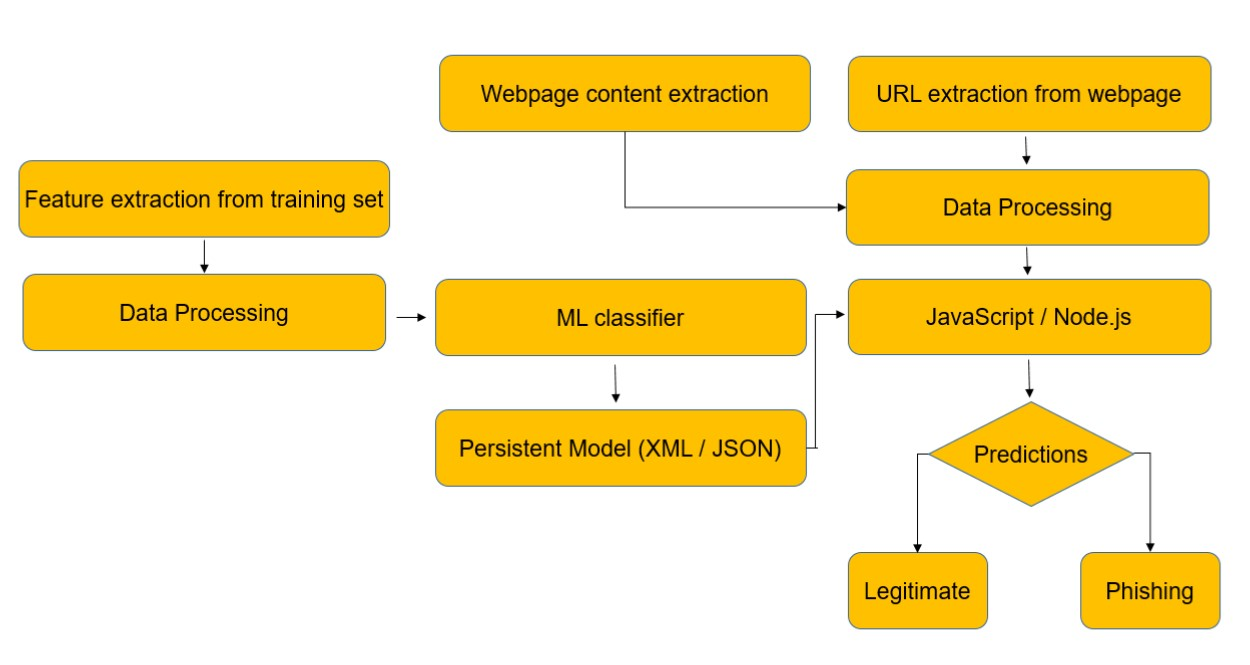
\includegraphics[width=\linewidth]{Fig1.jpg}
    \caption{Proposed phishing detection chrome extension
implementation}
    \label{fig:1}
\end{figure}
\section{Experimental Evaluation}
This project compares the performance of all the classifiers
described in section 5 on the phishing dataset. We have
evaluated these algorithms on 3317 test samples using various
performance metrics and this section contains the tabulated
results with their graphs.
\begin{table}[htp]
\caption{Random Forest Confusion Matrix}
\label{table:1}
\begin{tabular}{lcc}
\hline
                             & \begin{tabular}[c]{@{}c@{}}Predicted Phishing\\ URLs\end{tabular} & \begin{tabular}[c]{@{}c@{}}Predicted Legitimate\\ URLs\end{tabular} \\ \hline
Ground Truth Phishing URLs   & 1249                                                              & 162                                                                 \\
Ground Truth Legitimate URLs & 182                                                               & 1680                                                                \\ \hline
\end{tabular}
\end{table}
\par Table 1 shows the confusion matrix for Random forests.
With 1249 true positives, 182 false positives, 162 false
negatives and 1680 true negatives.
\begin{table}[htp]
\caption{Artificial Neural Network Confusion Matrix}
\label{table:2}
\begin{tabular}{lcc}
\hline
                             & \begin{tabular}[c]{@{}c@{}}Predicted Phishing\\ URLs\end{tabular} & \begin{tabular}[c]{@{}c@{}}Predicted Legitimate\\ URLs\end{tabular} \\ \hline
Ground Truth Phishing URLs   & 1205                                                             & 250                                                                \\
Ground Truth Legitimate URLs & 170                                                               & 1692                                                                \\ \hline
\end{tabular}
\end{table}
\par Table 2 shows the confusion matrix for Artificial neural
network. With 1205 true positives, 170 false positives, 250
false negatives and 1692 true negatives.
\begin{table}[htp]
\caption{SVM Confusion Matrix}
\label{table:3}
\begin{tabular}{lcc}
\hline
                             & \begin{tabular}[c]{@{}c@{}}Predicted Phishing\\ URLs\end{tabular} & \begin{tabular}[c]{@{}c@{}}Predicted Legitimate\\ URLs\end{tabular} \\ \hline
Ground Truth Phishing URLs   & 1293                                                             & 206                                                                \\
Ground Truth Legitimate URLs & 131                                                               & 1731                                                                \\ \hline
\end{tabular}
\end{table}
\begin{table}[htp]
\caption{Performance matrix of classifiers}
\label{table:4}
\begin{tabular}{lccc}
\hline
                          & Accuracy(\%) & Specificity(\%) & \multicolumn{1}{l}{Sensitivity(\%)} \\ \hline
Artificial Neural Network & 87.34        & 91              & 83                                  \\
Random Forest             & 89.63        & 90              & 86                                  \\
SVM                       & 89.84        & 93              & 89                                  \\ \hline
\end{tabular}
\end{table}
\begin{figure}
    \centering
    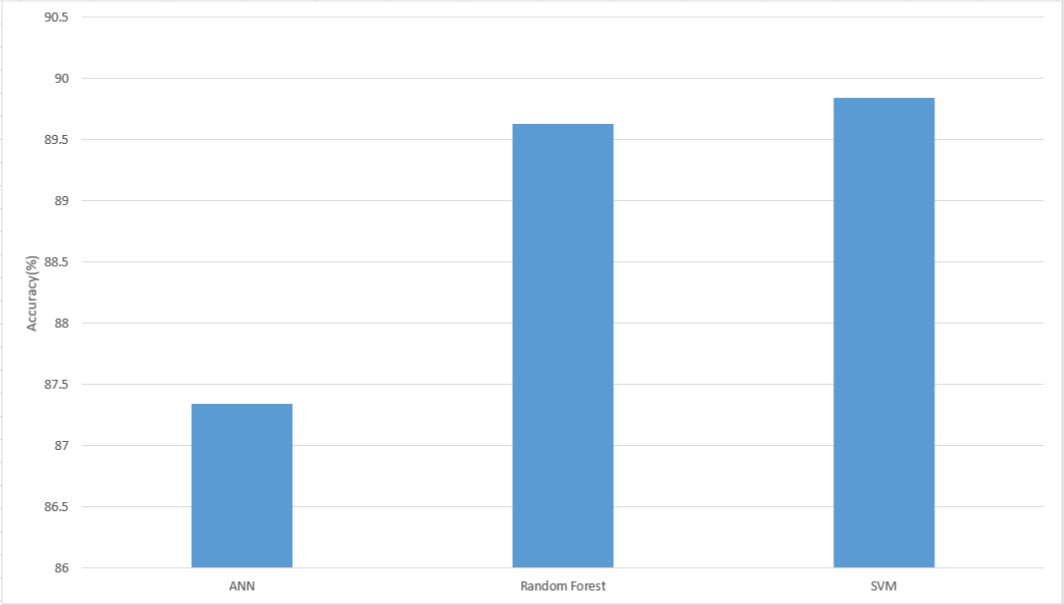
\includegraphics[width=\linewidth]{Fig2.jpg}
    \caption{Accuracy of classifiers}
    \label{fig:2}
\end{figure}
\begin{figure}
    \centering
    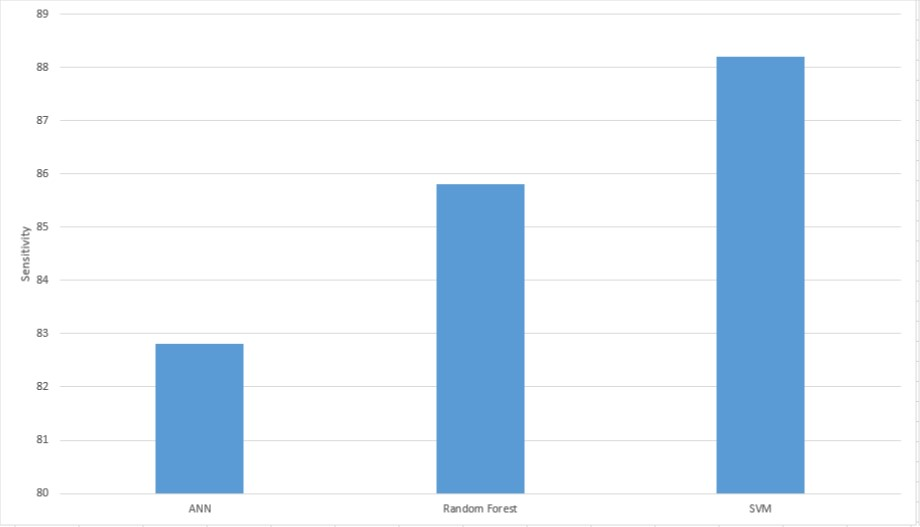
\includegraphics[width=\linewidth]{Fig3.jpg}
    \caption{Sensitivity of classifiers}
    \label{fig:3}
\end{figure}
\par Table 3 shows the confusion matrix for Support vector
machine. With 1293 true positives, 206 false positives, 131
false negatives and 1731 true negatives.
\par The Figure 2 shows the accuracy of each classifier evaluated
on 3317 test samples. From the above figure, it can be
seen that SVM outperforms all the other algorithms based on
accuracy in detection of Phishing URL. Also, Figure 3 shows
the sensitivity of each classifier. Here sensitivity refers to the
classifier’s ability to correctly detect phishing URLs. It can be
seen that SVM has the highest sensitivity among all the other
classifiers. However, in phishing detection, false positives and
false negatives are given more consideration when studying
the performance (predictive accuracy) of a classifier. That is
because false positives are more expensive than false negatives
in the real world. Since we do not want to allow users to
access the phishing URLs, false positives are considered to
be important while deciding the best classifier. The Figure 4
shows the false positive rates of all the classifiers. It is evident
that SVM has the least False positive rate among the three.
Hence, SVM works best in classifying the phishing URL from
the legitimate URLs.
\section{conclusion}
Thus to summarize, we have seen how phishing is a huge
threat to the security and safety of the web and how phishing
\begin{figure}
    \centering
    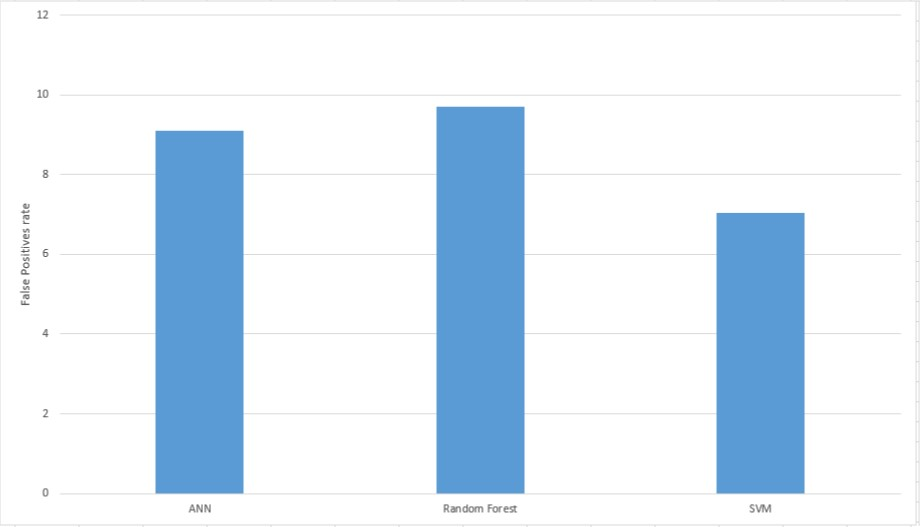
\includegraphics[width=\linewidth]{Fig4.jpg}
    \caption{False positive rate of classifiers}
    \label{fig:4}
\end{figure}
detection is an important problem domain. We have reviewed
some of the traditional approaches to phishing detection;
namely blacklist and heuristic evaluation methods, and their
drawbacks. We have tested three machine learning algorithms
on the ‘Phishing Websites Dataset’ from the UCI Machine
Learning Repository and reviewed their results. We then selected
the best algorithm based on it’s performance and built
a Chrome extension for detecting phishing web pages. The
extension allows easy deployment of our phishing detection
model to end users. For future enhancements, we intend to
build the phishing detection system as a scalable web service
which will incorporate online learning so that new phishing
attack patterns can easily be learned and improve the accuracy
of our models with better feature extraction.

% An example of a floating figure using the graphicx package.
% Note that \label must occur AFTER (or within) \caption.
% For figures, \caption should occur after the \includegraphics.
% Note that IEEEtran v1.7 and later has special internal code that
% is designed to preserve the operation of \label within \caption
% even when the captionsoff option is in effect. However, because
% of issues like this, it may be the safest practice to put all your
% \label just after \caption rather than within \caption{}.
%
% Reminder: the "draftcls" or "draftclsnofoot", not "draft", class
% option should be used if it is desired that the figures are to be
% displayed while in draft mode.
%
%\begin{figure}[!t]
%\centering
%\includegraphics[width=2.5in]{myfigure}
% where an .eps filename suffix will be assumed under latex, 
% and a .pdf suffix will be assumed for pdflatex; or what has been declared
% via \DeclareGraphicsExtensions.
%\caption{Simulation Results}
%\label{fig_sim}
%\end{figure}

% Note that IEEE typically puts floats only at the top, even when this
% results in a large percentage of a column being occupied by floats.


% An example of a double column floating figure using two subfigures.
% (The subfig.sty package must be loaded for this to work.)
% The subfigure \label commands are set within each subfloat command, the
% \label for the overall figure must come after \caption.
% \hfil must be used as a separator to get equal spacing.
% The subfigure.sty package works much the same way, except \subfigure is
% used instead of \subfloat.
%
%\begin{figure*}[!t]
%\centerline{\subfloat[Case I]\includegraphics[width=2.5in]{subfigcase1}%
%\label{fig_first_case}}
%\hfil
%\subfloat[Case II]{\includegraphics[width=2.5in]{subfigcase2}%
%\label{fig_second_case}}}
%\caption{Simulation results}
%\label{fig_sim}
%\end{figure*}
%
% Note that often IEEE papers with subfigures do not employ subfigure
% captions (using the optional argument to \subfloat), but instead will
% reference/describe all of them (a), (b), etc., within the main caption.


% An example of a floating table. Note that, for IEEE style tables, the 
% \caption command should come BEFORE the table. Table text will default to
% \footnotesize as IEEE normally uses this smaller font for tables.
% The \label must come after \caption as always.
%
%\begin{table}[!t]
%% increase table row spacing, adjust to taste
%\renewcommand{\arraystretch}{1.3}
% if using array.sty, it might be a good idea to tweak the value of
% \extrarowheight as needed to properly center the text within the cells
%\caption{An Example of a Table}
%\label{table_example}
%\centering
%% Some packages, such as MDW tools, offer better commands for making tables
%% than the plain LaTeX2e tabular which is used here.
%\begin{tabular}{|c||c|}
%\hline
%One & Two\\
%\hline
%Three & Four\\
%\hline
%\end{tabular}
%\end{table}


% Note that IEEE does not put floats in the very first column - or typically
% anywhere on the first page for that matter. Also, in-text middle ("here")
% positioning is not used. Most IEEE journals/conferences use top floats
% exclusively. Note that, LaTeX2e, unlike IEEE journals/conferences, places
% footnotes above bottom floats. This can be corrected via the \fnbelowfloat
% command of the stfloats package.




% conference papers do not normally have an appendix


% use section* for acknowledgement





% trigger a \newpage just before the given reference
% number - used to balance the columns on the last page
% adjust value as needed - may need to be readjusted if
% the document is modified later
%\IEEEtriggeratref{8}
% The "triggered" command can be changed if desired:
%\IEEEtriggercmd{\enlargethispage{-5in}}

% references section

% can use a bibliography generated by BibTeX as a .bbl file
% BibTeX documentation can be easily obtained at:
% http://www.ctan.org/tex-archive/biblio/bibtex/contrib/doc/
% The IEEEtran BibTeX style support page is at:
% http://www.michaelshell.org/tex/ieeetran/bibtex/
%\bibliographystyle{IEEEtran}
% argument is your BibTeX string definitions and bibliography database(s)
%\bibliography{IEEEabrv,../bib/paper}
%
% <OR> manually copy in the resultant .bbl file
% set second argument of \begin to the number of references
% (used to reserve space for the reference number labels box)
\begin{thebibliography}{1}

\bibitem{b1} Microsoft, Microsoft Consumer safety report. Available at
https://news.microsoft.com/en-sg/2014/02/11/microsoft-consumersafety-
index-reveals-impact-of-poor-online-safety-behaviours-insingapore/
sm.001xdu50tlxsej410r11kqvksu4nz

\bibitem{b2} Internal Revenue Service, IRS E-mail Schemes. Available at
https://www.irs.gov/uac/newsroom/consumers-warned-of-new-surgein-
irs-email-schemes-during-2016-tax-season-tax-industry-also-targeted

\bibitem{b3} Abu-Nimeh, S., Nappa, D., Wang, X., Nair, S. (2007), A comparison of
machine learning techniques for phishing detection. Proceedings of the
Anti-phishing Working Groups 2nd Annual ECrime Researchers Summit
on - ECrime ’07. doi:10.1145/1299015.1299021

\bibitem{b4} E., B., K., T. (2015)., Phishing URL Detection: A Machine Learning
and Web Mining-based Approach. International Journal of Computer
Applications,123(13), 46-50. doi:10.5120/ijca2015905665

\bibitem{b5} Wang Wei-Hong, L V Yin-Jun, CHEN Hui-Bing, FANG Zhao-Lin., A
Static Malicious Javascript Detection Using SVM, In Proceedings of
the 2nd International Conference on Computer Science and Electrical
Engineering(ICCSEE 2013)

\bibitem{b6} Ningxia Zhang, Yongqing Yuan, Phishing Detection Using Neural Network,
In Proceedings of International Conference on Neural Information
Processing, pp. 714–719. Springer, Heidelberg (2004)

\bibitem{b7} Ram Basnet, Srinivas Mukkamala et al, Detection of Phishing Attacks: A
Machine Learning Approach, In Proceedings of the International World
Wide Web Conference(WWW), 2003

\bibitem{b8} Sci-kit learn, SVM library. Available: http://scikitlearn.
org/stable/modules/svm.html

\bibitem{b9} Sklearn, ANN library. Available: http://scikitlearn.
org/stable/modules/ann.html

\bibitem{b10} Sklearn, Random foresets library. Available: http://scikitlearn.
org/stable/modules/Randomforesets.html

\bibitem{b11} Lichman, M. (2013). UCI Machine Learning Repository, University
of California, Irvine, School of Information and Computer Sciences.
Available: http://archive.ics.uci.edu/ml

\end{thebibliography}




% that's all folks
\end{document}


